
\section{PG-LDPC Implementation on un-partitioned/partitioned NoC}

%%%%%%% Insert Tanner Graph diagram and its explanation
\subsection{Tanner Graph formation}
\begin{frame}
\frametitle{Tanner Graph for PG-LDPC (7,3)}   % Insert frame title between curly braces
\begin{columns}[c]
\column{2.5in}  % slides are 3in high by 5in wide
\begin{itemize}
	\item PG-LDPC (7,3) code which is obtained by Projective Geometry over $GF(2^{s}),\ s=1$.
	\item The degree of total bit-node and check-node is $2^{s} +1 =3$.
	\item In this design, 5 bit precision :1 bit for sign, 3 bit of integer precision and 1 bit of fraction precision
\end{itemize} 

\column{2.5in}
\begin{center}
  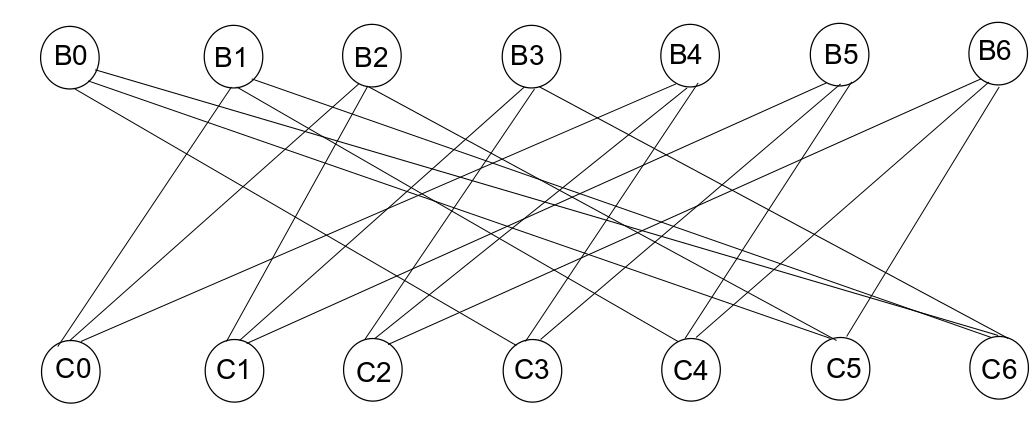
\includegraphics[scale=0.2]{./diagram/tanner_graph}
  Bn: Bit node n\\
  Cn: Check Node n
  \end {center}
  \end{columns}
\end{frame}


\begin {frame}
    \frametitle{How LDPC works?}
	  \begin{enumerate}
	  \item Initialize all bit nodes by Log Likelihood Ratio.
	  \item LLR propagates from bit nodes to check nodes via edges.
	  \item Check node performs computation.
	  \item Check node sends the computed LLR back to Bit node via edges.
	  \item Bit node checks whether the minimum required error is achieved or not.
	  \item If yes, sends the decoded data out, or else go to step(2).
	  \end{enumerate} 
\end {frame}

\subsection{Bit-Flipping Algorithm}
\begin{frame}
\frametitle{The Algorithm}   % Insert frame title between curly braces
A very simple explanation of bit-flipping algorithm is as follows
\begin{itemize}
	\item Check node bits are \textit{satisfied} if the sum of adjacent variable nodes is zero, \textit{unsatisfied} otherwise.
	\item Bit nodes flip the received value if the number of unsatisfied neighbours is larger than the number of satisfied neighbours.
\end{itemize}
\end{frame}



\subsection{PG-LDPC (7,3) Implementation using NoC}
\begin{frame}
\frametitle{System Implementation of PG-LDPC (7,3) using NoC}
\begin{columns}[c]
\column{2.2in}  % slides are 3in high by 5in wide
\begin{center}
Implementation on Mesh 4x4 un-partitioned NoC
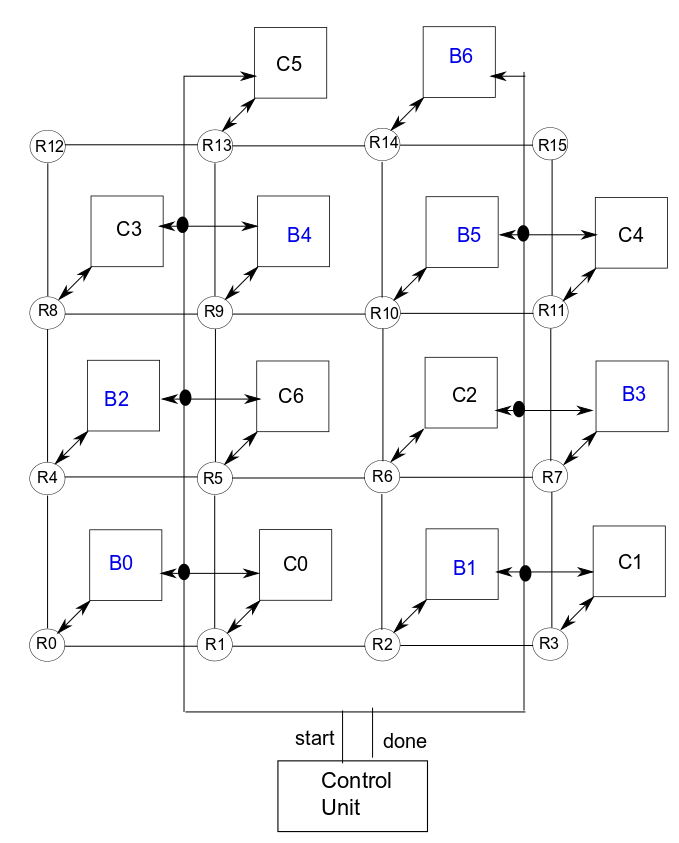
\includegraphics[scale=0.16]{./diagram/ldpc_7x7_noc_mesh_4x4}
\end{center}
\column{2.4in}
\begin{center}
Implementation on Mesh 4x4 partitioned NoC
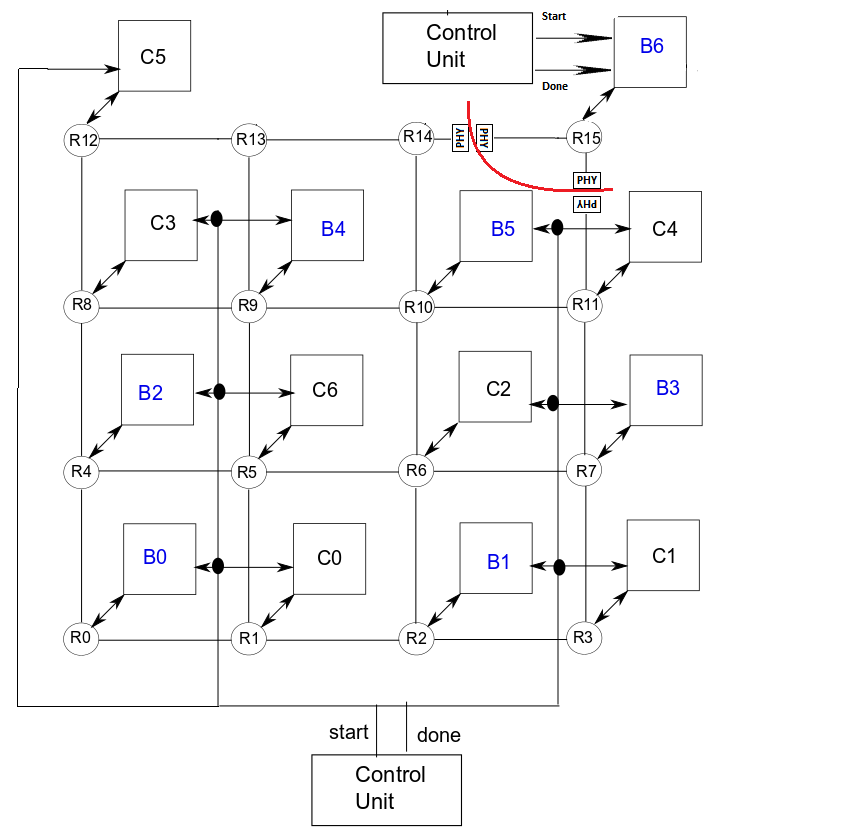
\includegraphics[scale=0.18]{./figs/Partitioned4X4Mesh}
\end{center}
\end{columns} 
\end{frame}

\subsection{Results and Comparison}
\begin {frame}
\frametitle {LDPC over NoC Flit Structure}
\begin{center}
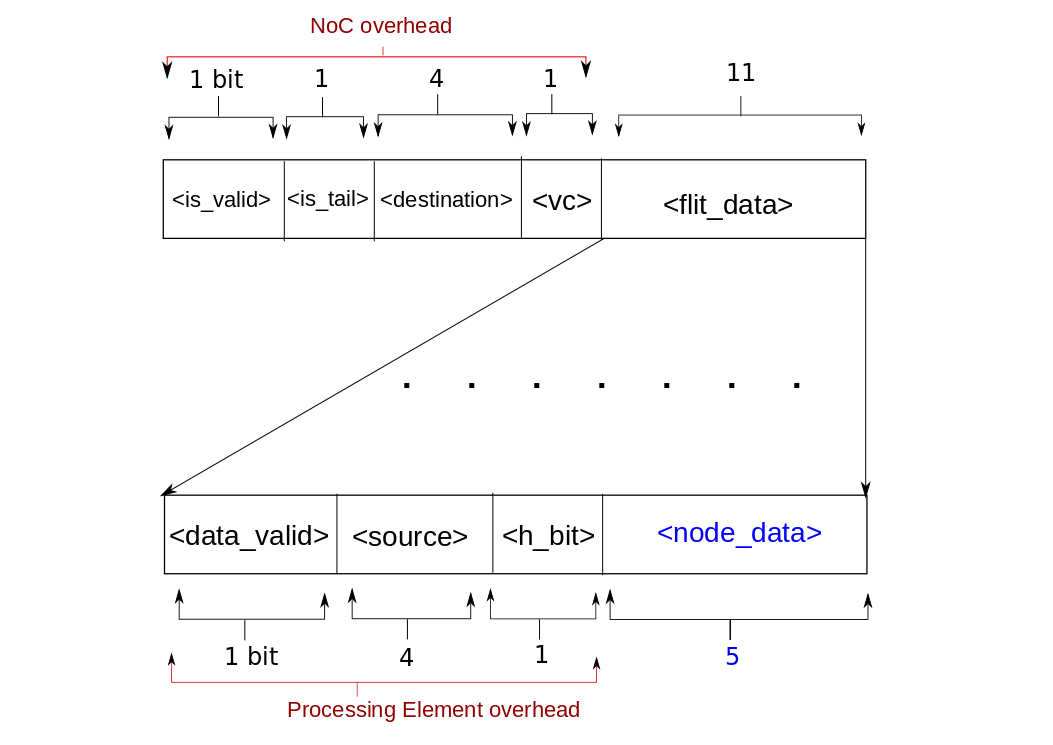
\includegraphics[scale=0.22]{./diagram/flit_structure_ldpc_7x7}
\end{center}

\end {frame}

\begin{frame}
\frametitle{Result comparison of Implementation of PG-LDPC(7,3) on un-partitioned NoC and partitioned NoC}
\begin{table} [scale=0.6]
\begin{center}
\resizebox{\textwidth}{!}
{\begin{tabular}{||c || c| c ||} \hline
Parameters 			      	& LDPC on 4$\times$4      	& LDPC on 4$\times$4 	\\ [0.5ex]
					& Mesh un-partitioned NoC 	& Mesh partitioned NoC  \\ \hline
Clock-cycle (1 iteration) 	      	& 18 				& 18+12\footnotemark	\\ \hline
Clock-cycle (n iteration) 	      	& 18 				& 18+12\footnotemark 	\\ \hline
Total cycle for n complete iteration 	& 18 + (n-1)$\times$12 		& (18 + (n-1)$\times$12) +12 \\ \hline
\end{tabular}}
\end{center}
\end{table}
\begin{center}
$Data Rate = \frac {Maximum\ frequency \times Data-width }{Nos\ of\ Iteration \times Nos\ of\ clock\ cycles} $.\\
\end {center}
\tiny
\textit{1,2:Whenever any data sent or received to or from partitioned node in this case for flit sent or received from bit node 15, additional 12 clock cycles is needed for the expected data to be received.}
\end{frame}

\begin{frame}
\frametitle{Performance Comparison and Resource Utilization for Altera :EP4CE22F17C6} 
\tiny
\begin{table} [scale=0.6]
\begin{center}
{\begin{tabular}{|| c || c | c | c ||}
\hline
				& Available  	& LDPC $7\times7$ Un-   & LDPC $7\times7$ 			\\ 
				& Resources  	& Partitioned      	& Partitioned Mesh 				\\
				&		& Mesh $4\times4$ NoC 	& $4\times4$ NoC				\\ \hline
	Number of		& 22,320     	& 9,840      	      	& 15,771 (71\%) (Part1) 			\\ 
	Logic Elements		&		& (44\%)		& 2,291  (10\%) (Part2)				\\ \hline
	Number of 		& 22,320     	& 6,651	              	& 11,113 (50\%) (Part1)				\\ 
	Logic Registers		&		& (30\%) 	      	& 1,787  (8 \%) (Part2)				\\ \hline
	Maximum Operating	& -          	& 36.27 MHz           	& 23.99 MHz 	(Part1)				\\  
	Frequency		&            	&                     	& 85.49 MHz	(Part2)				\\ \hline
	Number of clock		& -          	& 18                  	& 18 + 12(Part1)\footnotemark		\\ 
	cycles			&		&			& 18 + 12(Part2)\footnotemark		\\ \hline
	Data Rate		& -		& 36.27 Mbps		& 14.5 Mbps      				\\ \hline
\end{tabular}}
\end{center}
\end{table}

\tiny
\textit{1,2:Whenever any data sent or received to or from partitioned node in this case for flit sent or received from bit node 15, additional 12 clock cycles is needed for the expected data to be received.}
\end{frame}


  
  
  
